\documentclass[11pt]{extarticle}

\usepackage[sc]{mathpazo} 
\usepackage[spanish, es-tabla]{babel}
\usepackage[utf8]{inputenc}

\usepackage[hmarginratio=1:1,top=22mm, bottom=5mm,columnsep=20pt]{geometry} % Document margins
\usepackage{multicol} % Used for the two-column layout of the document
\usepackage[hang, small,labelfont=bf,up,textfont=it,up]{caption} % Custom captions under/above floats in tables or figures
\usepackage{mathtools}
\usepackage{float} % Required for tables and figures in the multi-column environment - [H] needed
\usepackage{hyperref} % For hyperlinks in the PDF with labels

\usepackage{abstract} % Allows abstract customization
\renewcommand{\abstractnamefont}{\normalfont\bfseries} % Set the "Abstract" text to bold
\renewcommand{\abstracttextfont}{\normalfont\small\itshape} % Set the abstract itself to small italic text

\newcommand{\mudeb}{\textbf{MuDeb} }

\usepackage{titlesec} % Allows customization of titles
\usepackage{pdfpages}
\usepackage{multirow}
\usepackage{array}

\titleformat{\section}[block]{\huge\scshape\bfseries}{\thesection.}{1em}{} % Change the look of the section titles
\titleformat{\subsection}[block]{\Large}{\thesubsection.}{1em}{} % Change the look of the section titles

\usepackage{fancyhdr} % Headers and footers
\pagestyle{fancy} % All pages have headers and footers
\fancyhead{}
\fancyfoot{} % Blank out the default footer
\fancyhead[C]{MuDeb% based on TRACS 
\hspace{10pt} $\bullet$ \hspace{10pt} Jaime Díez González-Pardo \hspace{10pt} $\bullet$ \hspace{10pt} Abril 2019 \hspace{10pt}} % Custom header text
\fancyfoot[RO,LE]{\thepage} % Custom footer text

%----------------------------------------------------------------------------
%      · DOCUMENT
%----------------------------------------------------------------------------

\begin{document}


	%\maketitle % Insert title

	\begin{titlepage}
		\begin{center}

			\vspace{-10cm}

			
\includegraphics[width=0.4\textwidth]{Fotos/Logo/logoFinal.png}\\[1cm]

			%{\large Intitulé de la filière, domaine ou approfondissement}\\[0.5cm]

			%{\large Type de projet}\\[0.5cm]

			% Title
			\rule{\linewidth}{0.5mm} \\[0.4cm]
			{\bfseries \Huge{\mudeb} \huge Red de difusión de Física de Partículas \\[0.4cm] }
			\rule{\linewidth}{0.5mm} \\[1.5cm]

			\begin{abstract}

				\noindent% Dummy abstract text

					El objetivo de este proyecto es el diseño de un experimento de detección de muones cósmicos que permita ser reproducido de manera sencilla y barata en institutos y universidades. Para ello será necesario el desarrollo del dispositivo experimental, así como el de una red que permita acceder a ciertos datos del experimento desde cualquier parte del mundo tomados en tiempo real. Con ello, se pretende divulgar la física de partículas a jovenes con conocimientos básicos en física, pudiendo realizarse el experimento en aulas sin necesidad de dispositivos complejos.

			\end{abstract}

			\vspace{1cm}

			\textbf{Participantes}

			\begin{table}[H]
				\centering
				\begin{tabular}{ c c l c c c}
					\centering
						Participante 	& & Nombre 							&					& & Filiación 				\\
										& &									&					& &							\\ 
						1 (Coordinador) & & Jaime Díez González-Pardo 		& \textbf{(JDGP)}	& & 4º Física 				\\ 
						2 				& & Marcos Seror García 			& \textbf{(MSG)}	& & Lincenciado en Física 	\\ 
						3 				& & Patricia Marín Ruiz del Haya 	& \textbf{(PMRH)}	& & Doctora en Física 		\\ 
						4 				& & Laura Lloret Iglesias 			& \textbf{(LLI)}	& & Doctora en Física 		\\ 
						5 				& & Roberto Vilar Cortale 			& \textbf{(RVC)}	& & Doctor en Física 		\\ 
						6 				& & Daniela Iglesias Sánchez		& \textbf{(DIS)}	& & 4º Física 				\\ 
				\end{tabular}
			\end{table}

			\vfill

			% Bottom of the page
			%{\large Version 0.1 du\\ \today}

		\end{center}
	\end{titlepage}


%----------------------------------------------------------------------------
%	  ABSTRACT
%----------------------------------------------------------------------------

	\newgeometry{hmarginratio=1:1, top=32mm, bottom=25mm,columnsep=40pt}
	\thispagestyle{fancy} % All pages have headers and footers
	\newpage
	\renewcommand{\abstractname}{Resumen Ejecutivo}
	\begin{abstract}

		\noindent

			\mudeb es un proyecto de difusión de la física de partículas en institutos y universidades orientado a jovenes con conocimientos básicos en física. Para ello se centrará en diseñar el experimento de la medida de la vida media del muón y la dilatación temporal a partir de la detección de la desintegración de muones cósmicos, de manera que resulte fácil reproducirlo. Para lograr el objetivo el proyecto se centrará en el desarrollo del dispositivo experimental y la red de datos, que permita realizar el experimento desde cualquier lugar, así como de la difusión del proyecto en universidades e intitutos de todo el mundo. \\

			La física de partículas es en ocasiones denominada como física de altas energías debido a la gran complejidad de sus experimentos (LHC, Super Kamiokande o Tevatrón son algunos de los ejemplos), que requieren ser realizados en condiciones de gran energía. Esta gran escala de sus experimentos, junto con la complejidad de los fundamentos teóricos en los que se sustenta, hacen que resulte dificil su divulgación, o que ésta se base en simulaciones o resultados de medidas pasadas que ya han sido analizadas y procesadas. Esto elimina la interacción directa del público con el objeto de estudio y resultan mucho menos atractivas que aquellas que se basan en observaciones directas. Algunos ejemplos de esto son las \textit{MasterClasses Hands On Particle Physics} realizadas por el Grupo Internacional de Divulgación de Física de Partículas (\textit{International Particle Physics Outreach Group}, \textbf{IPPOG}), utilizando los datos del LHC, y que en ocasiones se ha reproducido en grados de física como prácticas de laboratorio.\\

			Por dicho motivo se ha escogido el experimento de la medida de la vida media del muón, que se realiza a partir de muones cósmicos creados en la atmósfera y que llegan constantemente a la superficie de la Tierra. Esto produce una gran dismunición de la complejidad del dispositivo experimental al no ser necesario la creación de dichas partículas y tener una alta probabilidad de detección. Además, el fundamento teórico de este experimento es la ley de desintegración exponencial, de gran simplicidad y que no requiere de grandes conocimientos previos en física de partículas y de una abstracción mental compleja, por lo que puede ser comprensible para el alumnado de Bachillerato. Por otro lado, también permite profundizar más en la física de partículas en temas más complejos a medida que el conocimiento base aumenta, por lo que es idóneo no solo para su divulgación sino que además puede ser realizado como prácticas de laboratorio del grado en física.\\

			Para la realización del experimento se desarrollaran dos dispositivos experimentales para la detección de la desintegración de los muones, contando con una versión básica y otra autónoma. La versión básica del dispositivo experimental incluirá todo lo necesario para realizar el experimento en aulas y será el que se utilice en las jornadas de difución. Por otro lado, la versión autónoma estará diseñada para poder ser utilizada de forma remota sin necesidad de estar conectada a la corriente. Este último dispositivo formará parte de una red de dispositivos situados por todo el mundo a diferentes alturas y será utilizado de forma remota durante las jornadas de difusión a través de una página web.\\

			El proyecto se realizará en colaboración con el Instituto de Física de Cantabria (\textbf{IFCA}) que en la actualidad cuenta con una importante actividad en el área de divulgación, participando en actividades del \textbf{IPPOG}, y que ha sido acreditado como centro de excelencia María Maeztu. El \textbf{IFCA} facilitará personal, presupuesto y estructura empresarial necesaria. Además, se utilizarán sus colaboraciones con centros de investigación y universidades de todo el mundo para la difusión y colaboración del proyecto.

	\end{abstract}


	\newpage
	\tableofcontents
	\newpage

%----------------------------------------------------------------------------
%	  Proyect CONTENTS
%----------------------------------------------------------------------------

		\section{Presentación general de la propuesta}
			\addtocontents{toc}{\vspace{0.1cm}}
			\label{Sec:PreGeneral}

			\subsection{Objetivos}
				\addtocontents{toc}{\vspace{0.1cm}}
				\label{SubSec:PreGeneral:Obj}

				El objetivo del proyecto es la creación de una red de difusión de la física de partículas a través del experimento de la medida de la vida media del muon. Esta red de difusión se encargará de organizar eventos en institutos y universidades dedicados a jovenes alumnos con conocimientos básicos en física. En estas jornadas se realizará dicho experimento, impartiendo carlas formativas sobre la física del proyecto y facilitando a los participantes todo lo necesario para su realización.

				Para ello será necesario el desarrollo de los dispositivos experimentales que permitan obtener los datos de las desintegraciones de los muones. Puesto que para la completa realización del experimento es conveniente realizar las medidas a diferentes alturas y ante la complejidad de mover el experimento y a los participantes durante la realización de las jornadas, se desarrollará un dispositivo más complejo. Este dispositivo se autoabastecerá energéticamente, permitiendo tomar medidas en lugares remotos y acceder ellas via internet a través de una red de datos.

				El objetivo del desarrollo del dispositivo experimental autónomo es conseguir un dispositivo de medida de las desintegraciones de muones cósmicos que funcione de forma totalmente autónomo y permita acceder a sus datos de forma remota durante un periodo mínimo de cinco años. Se espera poder tener operativos tres de estos dispositivos en las zonas de Picos de Europa, Pirineos y el Macizo del Jura en un plazo de tres años, aumentando el número de puestos de tomas de datos en función de la colaboración de otro centros de investigación y universidades.

				El plazo marcado para el cumplimiento de los objetivos es de tres años, en el cuál se prevé haber realizado las jornadas de disusión en un total de 20 institutos y universidades de al menos 3 países diferentes.

			\subsection{Concepto y Metodología}
				\addtocontents{toc}{\vspace{0.1cm}}
				\label{SubSec:PreGeneral:ConcpMet}

				\subsubsection{El Experimento}
					\addtocontents{toc}{\vspace{0.1cm}}
					\label{SubSubSec:PreGeneral:ConcpMet:Exprmnt}

					El experimento que se pretende realizar durante las jornadas de divulgación es la medida de la vida media del muon (\textit{Measurement of the muon life time }\cite{guia}) en el cual se obtiene el valor de la vida media del muon a partir del tiempo de la desintegración del muon, $\tau$. Dicho experimento se realiza actualmente en el grado en física y forma parte de las prácticas realizadas en la asignatura Advanced Experimental Techniques del cuarto curso del grado en física de la universidad de Cantabria.

					En el experimento se estudia el decaimiento de los muones que se forman en la atmósfera provenientes de los rayos cósmicos en electrones y neutrinos. La probabilidad de que se produzca un decaimiento en un determinado tiempo viene dado por una ley exponencia cuyo parámetro es el tiempo de vida medio del muon. Así, midiendo el número de desintegraciones que se producen dentro del detector en un tiempo $t$ se ha de poder ajustar los datos a un ajuste exponencial que permita obtener $\tau$.

						\begin{multicols}{2}
							\[
								\mu^- \rightarrow e^- + \bar{\nu}_e + \bar{\nu}_\mu
							\]

							\[
								P(t) = e^{-t/(\gamma \tau)}
							\]
						\end{multicols}

					Pero este experimento no solo permite obtener el valor de la vida media del muon, sino que la medida de los decaimientos de los muones permite estudiar otro fenómenos que ocurren a la vez.

					De este modo, el experimento también permite obtener una demostración del efecto de dilatación temporal debido a la relatividad. Para ello, se estudian las relaciones entre las tasas de muones detenidos en el detector a dos alturas diferentes. Debido a la pérdida de energía que sufre el muon medido en el experimento a una altura más baja, la tasa de muones detenidos en el detecotor será menos, y dependerá del tiempo de tránsito desde la altura de uno de los experimentos al otro. 

					Se puede comprobar fácilmente como los valores de la relación entre tasas obtenidos de forma experimental se ajustan con una mayor compatibilidad a los resultados teóricos obtenidos teniendo en cuenta el efecto de dilatación temporal que con los resultados que se obtendrían sin la dilatación temporal.

						\begin{equation*}
							\begin{matrix}
								\textrm{Tiempo de tránsito en el sistema de referencia del muon con dilatación temporal}\\ \\
								t' \simeq \frac{mc}{\rho S_0} \int^{\gamma_1}_{\gamma_2} \frac{\textrm{d}\gamma}{\sqrt{\gamma^2 - 1}} \rightarrow S_0 = 2 MeV g^{-1} cm^{2} 
							\end{matrix}
						\end{equation*}

				\subsubsection{El Dispositivo}
					\addtocontents{toc}{\vspace{0.1cm}}
					\label{SubSubSec:PreGeneral:ConcpMet:disp}

					El instrumental utilizado para la realización del experiemento se basa en el dispositivo experimental desarrollado por Thomas Coan, Tiankuan Liu y Jingbo Ye \cite{physics/0502103} y comercializado por la empresa Teach Spin \cite{TeachSpin}. Dicho dispositivo fue desarrollado para su uso en laboratorios para pregraduados, y está formado por un detector, de plástico centelleador acoplado a un fotomultiplicador, y a una caja electronica de lectura. Dicho dispositivo necesita de un ordenador externo para la lectura de los datos por el usuario.

						\begin{figure}[H]
							\centering
							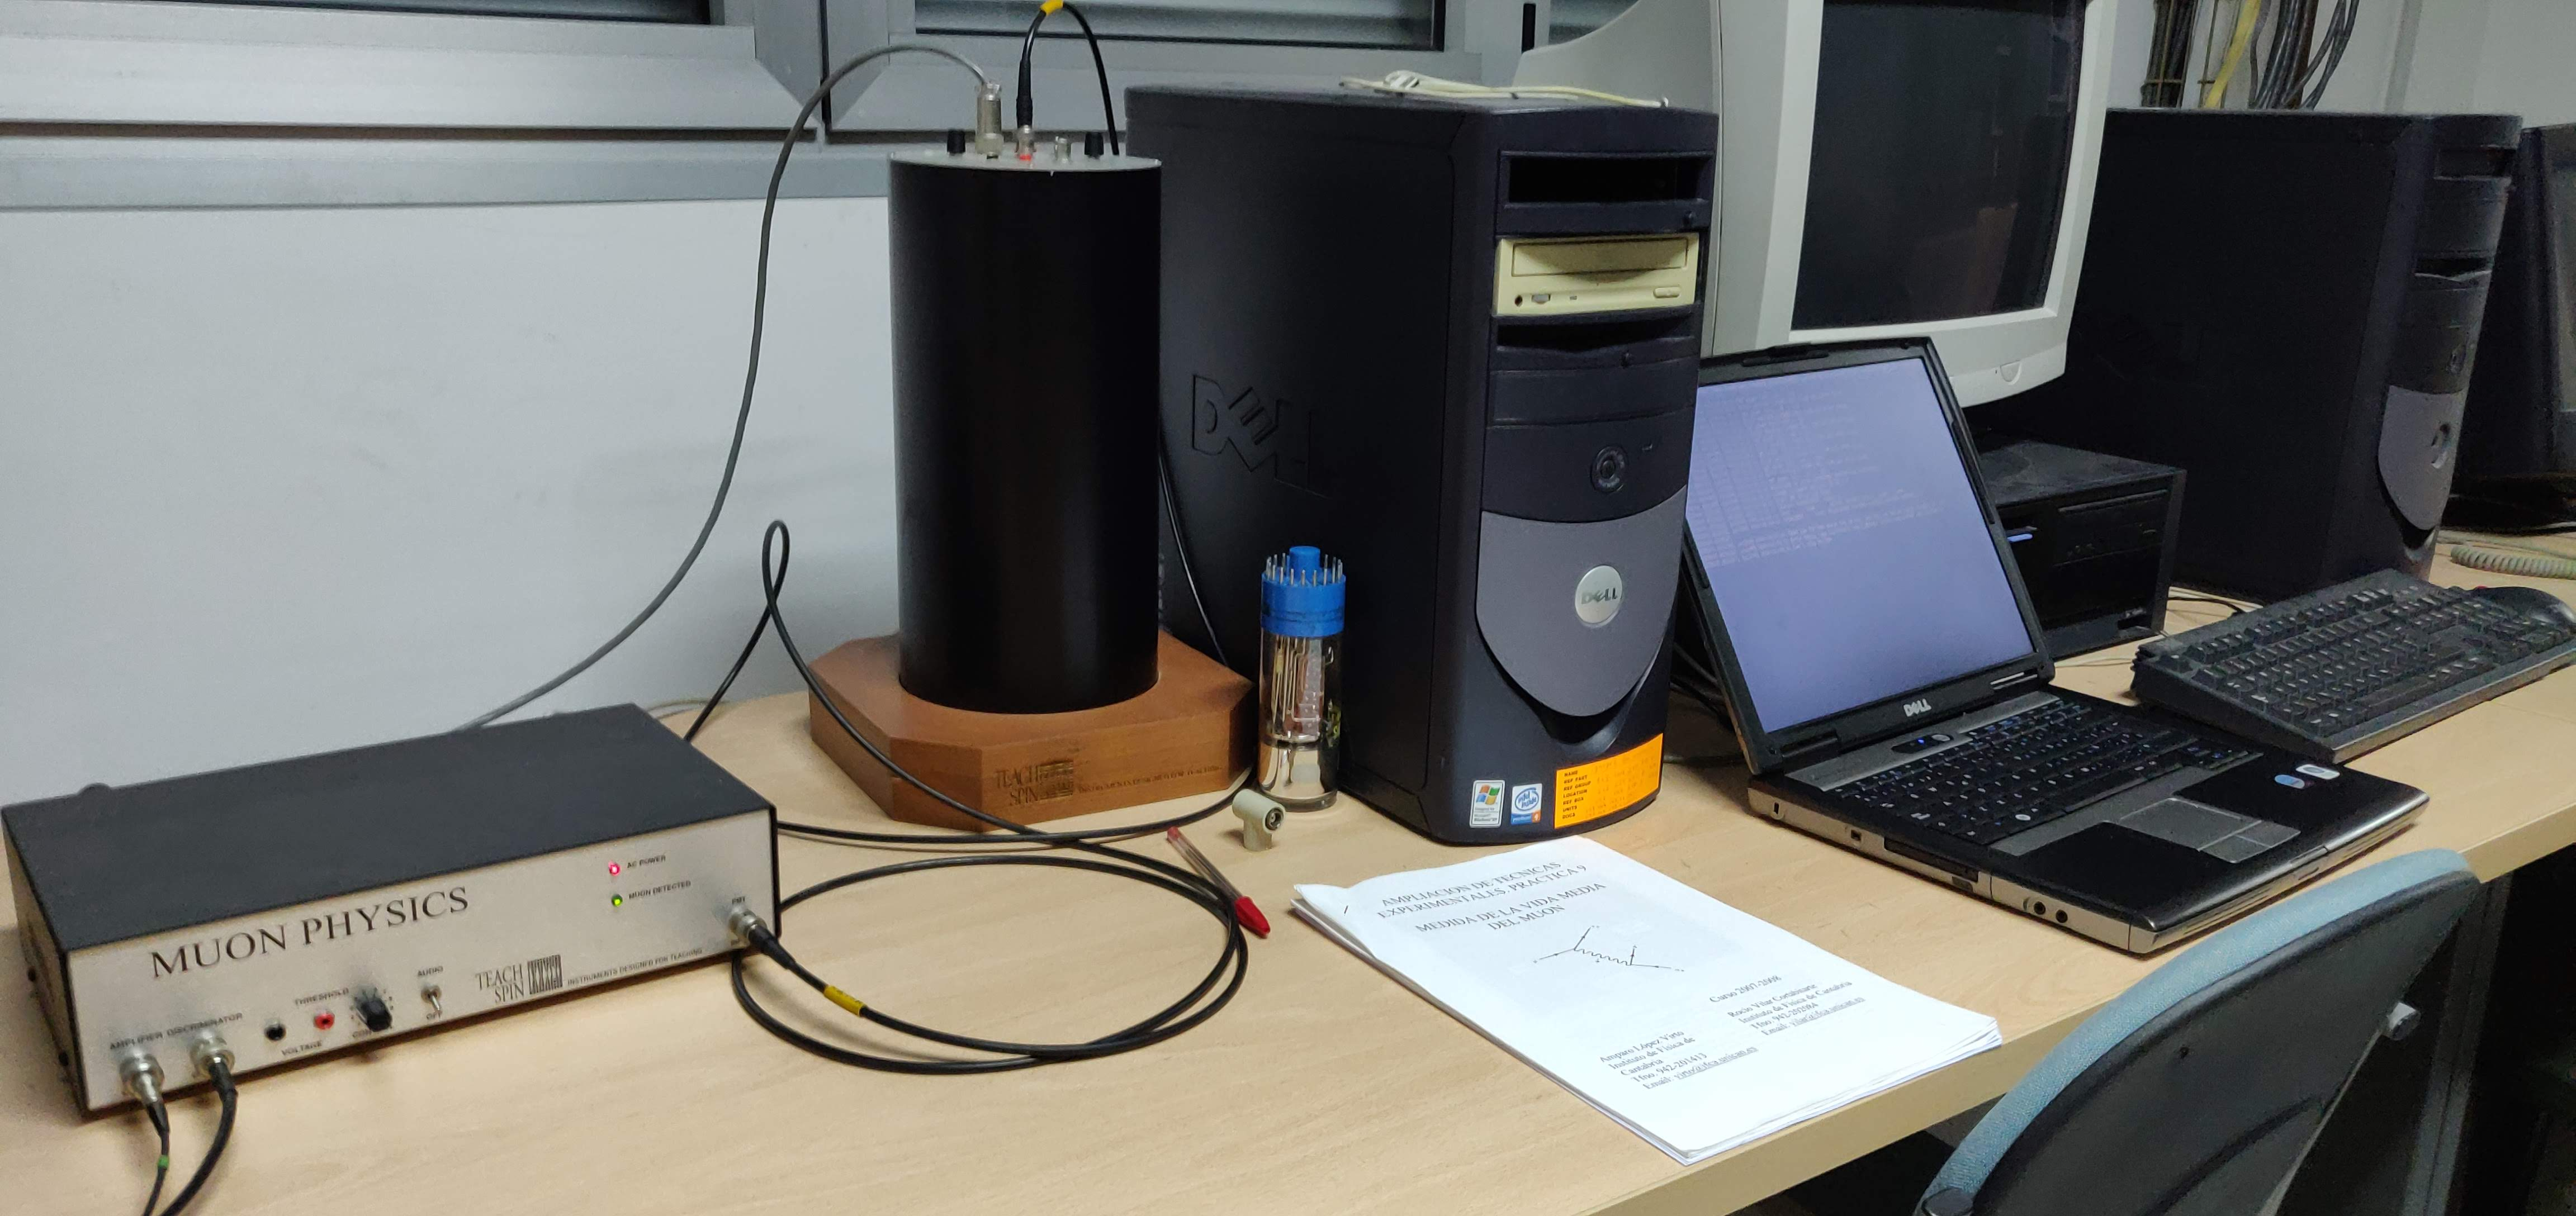
\includegraphics[scale=0.05]{Fotos/IMG_20180927_113646.jpg}
							\caption{\label{Img:widgets}Imagen del dispositivo experimental comercializado por Teach Spin y que se utiliza en la asignatura del grado en física de la universidad de cantabria.}
						\end{figure}

					La caja electronica de lectura obtiene el pulso de corriente proveniente del detector, si en una ventana de tiempo de 20 $\mu$s se produce otro pulso de corriente equivalente a la desintegración del muon en un electrón, devuelve la diferencia de tiempo entre ambos pulsos en unidades integrales del reloj de periodo 50 MHz. De no producirse un segundo pulso en la ventana de 20 $\mu$s, devuelve el valor 10000, que es el número de unidades integrales del reloj de periodo 50 MHz que hay en dicha ventana. De esta forma, la información que le transmite al ordenador es un número entero, que es tratado por el programa para convertirlo en el tiempo de la desintegración.

					La empresa Teach Spin suministra junto con el dispositivo el software necesario para la realización de la práctica. Sin embargo, para este rpoyecto se utilizará el software desarrollado en el \textbf{IFCA} para dicho experimento y que permite acceso a los dato de forma remota, siendo este programa de código abierto \cite{MULTIDAQ}.

					El modelo básico del dispositivo que se desarrollará y se utilizará en las jornadas de divulgación estará basado en el dispositivo comercializado por Teach Spin, realizando ciertos cambios que abaraten el dispositivo, lo hagan más compacto y manejable; e incluya un ordenador que permita utilizarlo sin necesidad de tener que instalar el programa de adquisición de datos en más odenadores.

					Por otro lado, se desarrollará un dispositivo más complejo al que se le incluirá paneles solares que permitan autoabastecer al dispositivo de energía. Además, contará con un sistema de comunicaciones half-duplex UHF transceiver que permitirá comunicar los datos recogidos por el dispositivo, siendo accesibles de forma remota. 

				\subsubsection{Estado del Arte}
					\addtocontents{toc}{\vspace{0.1cm}}
					\label{SubSubSec:PreGeneral:ConcpMet:StatArt}

					La actividad divulgativa en la rama de la física a crecido enormemente en los últimos años, siendo capaz de llegar a un mayor número de gente y captando año a año nuevos estudiantes. Por ello, los grandes centros de investigación han aumentado su implicación en este área, pomoviendo actos, jornadas y eventos dedicados a acercar la física y los experimentos al público, especialmente a los jovenes, potenciales científicos del futuro.

					Un claro ejemplo de esto es la gran actividad divulgativa del \textbf{CERN}, uno de los mayores centros de investigación del mundo, que organiza numerosos eventos de divulgación por todo el mundo. Cabe destacar especialmente su participación en las masterclasses \textit{Hands on Particle Physics} organizadas por \textbf{IPPOG} y que se realizan desde hace años en más de 55 paises diferentes.

					Esta actividad, junto con otras muchas actividades dedicadas a la divulgación, es realizada en el \textbf{IFCA}, cuya implicación en la divulgación científica junto con la universidad de cantabria, ha tenido un papel fundamental en el crecimiento de interés científico en los jovenes de la región. El \textbf{IFCA} participa activamente en numerosas actividades de divulgación como \textit{La Noche de los Investigadores}, \textit{Pint of Science}, \textit{Café Científico}, ...

				\subsubsection{Metodología}
					\addtocontents{toc}{\vspace{0.1cm}}
					\label{SubSubSec:}

					El proyecto se pretende llevar a cabo en cuatro fases distintas en función de la evolución del proyecto. La primera fase del proyecto consistirá en la investigación de toda la información necesaria para el desarrollor del proyecto. Una vez obtenida toda la información necesaria para el proyecto comenzará la fase de desarrollo. La prioridad en esta fase se centrará en el desarrollo y puesta a punto de los dos dispositivos experimentales necesarios para la realización del experimento en las jornadas de divulgación. Por otro lado, también será necesario el desarrollo informático de la red de datos que conecte los dispositivos y permita conectarse a ellos de manera remota. Una vez obtenido todo lo necesario para la realización de las jornadas de divulgación se realizarán dichos eventos por parte de los miembros del proyecto, desplazandose a universidades e intitutos, comenzando la actividad divulgadora del proyecto.

					Estas tres primeras fases del proyecto se esperan que duren un periodo de 3 años y sean el principal bloque del proyecto. Tras esto, se espera que la colaboración por parte de centros externos aumente, pudiendo ser realizadas las actividades por terceros, minimizando la actividad del grupo de proyecto, limitando su actividad a centro de la zona y coordinando los eventos realizados por centro externos.


				\subsubsection{Stakeholders}
					\addtocontents{toc}{\vspace{0.1cm}}
					\label{SubSubSec:}

					Al tratarse de un proyecto de divugación qque pretende ser realizado en centros externos y ser sustentado con la colaboración de otros centros, son varios los colectivos que se pueden ver afectados por el proyecto y de los que depende el éxito de este.

					\begin{itemize}
						\item \textbf{Universidad de Cantabria} Se pretende englobar el proyecto dentro de las actividades de divulgación que ya realiza la universidad y que servirían de impulso al comienzo del proyecto, por lo que es necesario un nivel de apoyo alto. Estas actividades ayudarían a mejorar la imagen de la universidad publicitando sus actividades de divulgación. También servirían para captar a futuros estudiantes de la universidad, por lo que se espera un nivel de apoyo total.

						\item \textbf{Institutos Educativos} Este proyecto está destinado a alumnos de bachillerato por lo que se intentaría vincular a actividades de los centro educativos que impartan el bachillerato, sirviendo como cauce de difusión entre el alumnado, por lo que se necesitaría un nivel de apoyo suficiente. Estas actividades supondrían una formación extra para su alumnado sin suponer un mayor esfuerzo por parte del centro, por lo que se espera un apoyo alto.
					\end{itemize}

			\subsection{Presentación del proyecto en el formato LogFrame}
				\addtocontents{toc}{\vspace{0.1cm}}
				\label{SubSec:PreGeneral:LogFram}

				\begin{figure}[H]
					\centering
					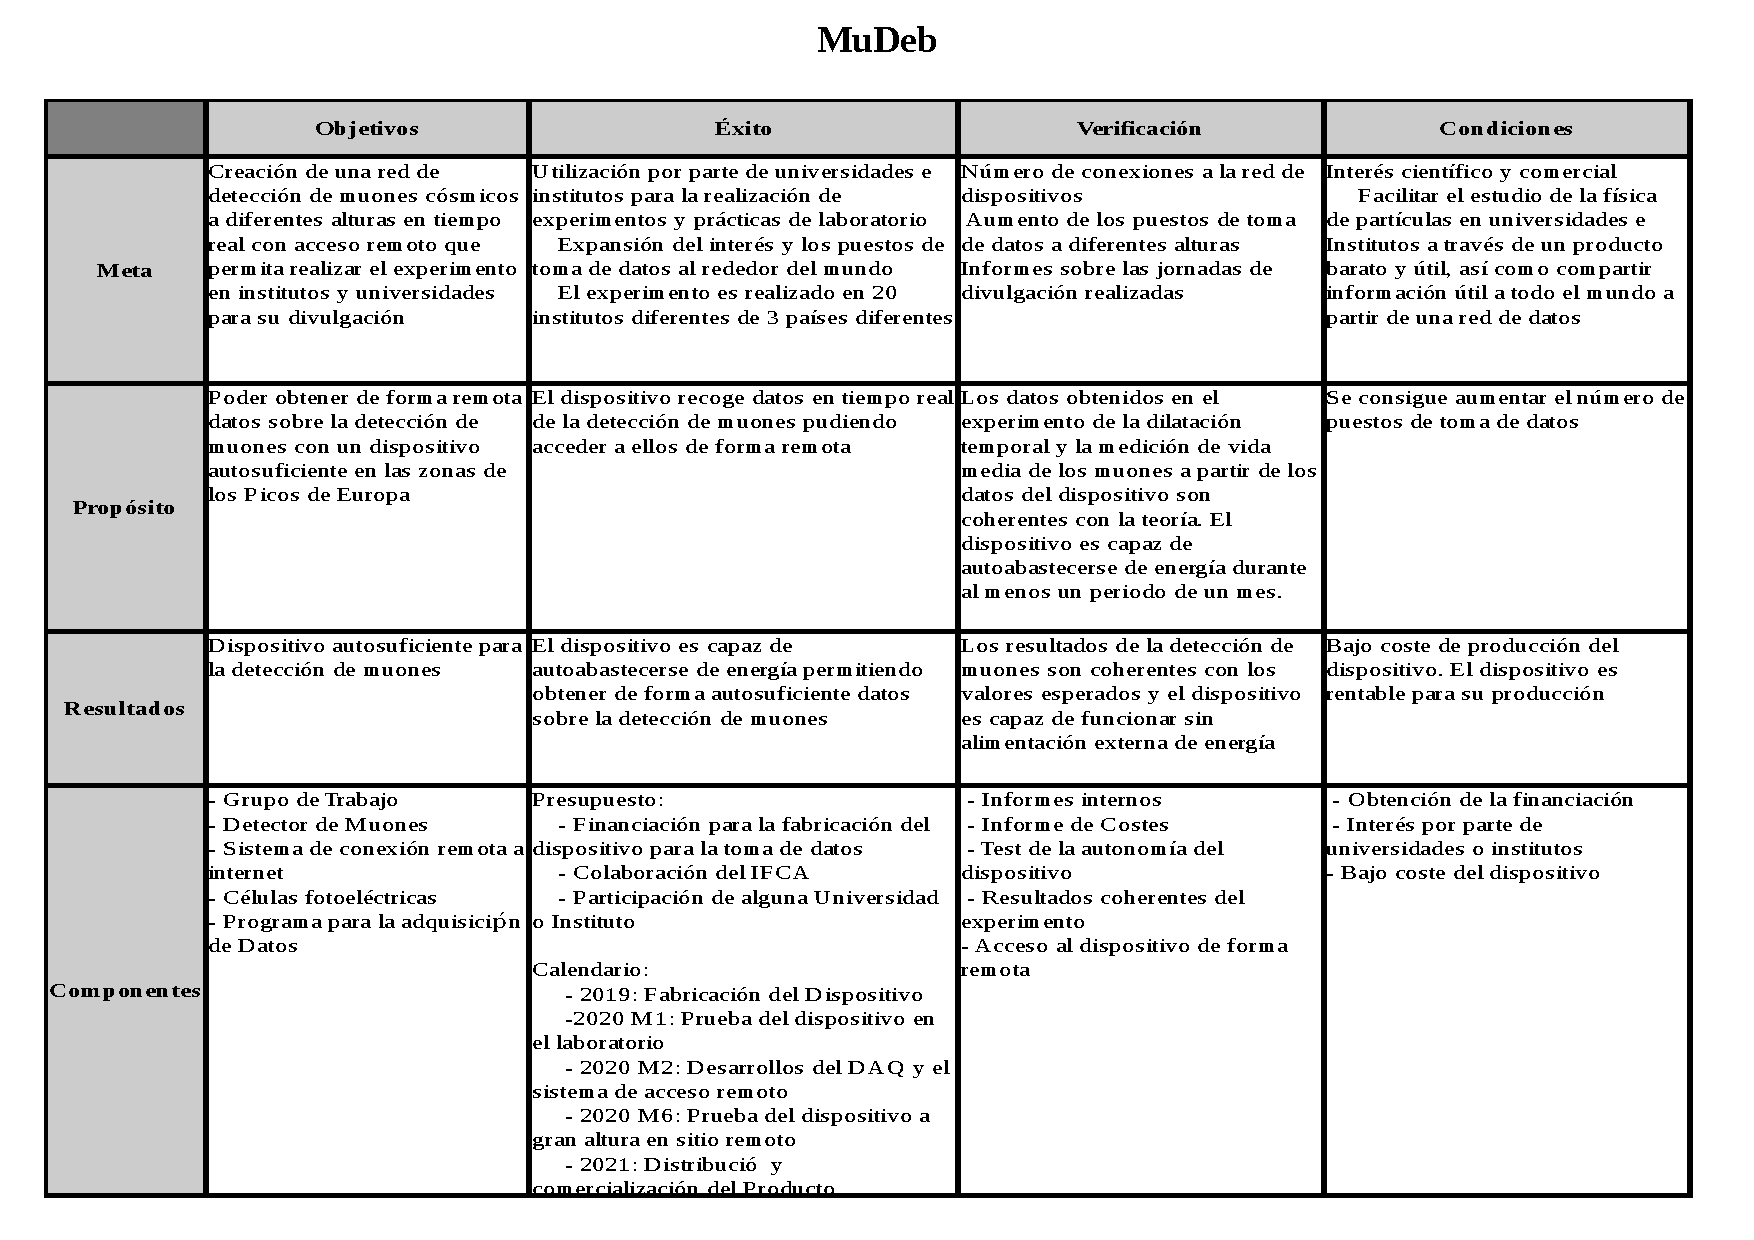
\includegraphics[scale=0.54]{LogFrameMudeb.pdf}
					\caption{\label{Img:widgets}Why not}
				\end{figure}

			\subsection{Ambición}
				\addtocontents{toc}{\vspace{0.1cm}}
				\label{SubSec:PreGeneral:Ambicion}
							 
				Pese a que en la actualidad son numerosos los expeerimentos de divulgación que se llevan a cabo en el área de la física, la física de partículas sigue teniendo un lastre con respecto a otras ramas de la física a la hora de llevar sus experimentos a institutos para captar alumnos. Este experimento permite llevar un gran conocimiento de la física de partículas a los alumnos de bachillerato, pudiendo experimentar en primera persona con partículas elementales.

				Además, este experimento permite ser modificado y apliado en función del conocimiento base del público al que va diriguido, pudiendo ser divulgado a diferentes niveles.
		
		
		\section{Implementación}
			\addtocontents{toc}{\vspace{0.1cm}}
			\label{Sec:Imple}

			\subsection{Plan de trabajo por fases}
				\addtocontents{toc}{\vspace{0.1cm}}
				\label{SubSec:Imple:trbjFases}

				El proyecto estará dividido en varias fases en función de la madured del mismo, pudiendo pasar de una fase a otra unicamente cuando ésta haya concluido.

				\begin{itemize}
					\item \textbf{Investigación} Los primeros tres meses del proyecto serán dedicados a la organización del proyecto en sus paquetes de trabajo, organigrama y trabajo de colaboración entre los diferentes paquetes de trabajo para la obtención de la información necesaria para realizar el proyecto. En esta primera fase se decidirán los plazos de trabajo, se llevará a un consenso sobre la metodología que se llevará a cabo durante las jornadas de divulgación, así como de todo el material que será necesario para ello.

					\item \textbf{Desarrollo} La fase principal del proyecto consistirá en el desarrollo del instrumental necesario para realizar el experimento y tendrá una duración de 15 meses. En esta fase se comenazará a colocar los primeros dispositivos remotos que constituyan la red de datos.

					\item \textbf{Divulgación} Una vez se disponga del material necesario para la realización del experimento se realizarán jornadas divulgativas en institutos y universidades, realizando un control sobre el éxito de las jornadas.

					\item \textbf{Fin} Tras año y medio realizando las jornadas de divulgación se estudiará la viabilidad del proyecto a trravés de la implicación de intitutos y centros externos.
				\end{itemize}

			\subsection{Descripción de los paquetes de trabajo}
				\addtocontents{toc}{\vspace{0.1cm}}
				\label{SubSec:Imple:WP}

					El la Tabla \ref{Tab:allWP} se muestran los diferentes paquetes de trabajo (\textit{Work package} WP) en los que está dividido el proyecto.

						\begin{table}[H]
							\centering
							\begin{tabular}{ c c c c c }
								\hline
								\centering
									Work Package 	& Nombre del WP 	& Coordinador 	& Comienzo del WP 	& Fin del WP \\ \hline
									\hline
									WP1 			& Coordinación 		& \textbf{JDGP} & 03/06/2019 		& 03/06/2022 \\ \hline
									WP2 			& Investigación 	& \textbf{PMRH} & 03/06/2019 		& 03/09/2019 \\ \hline
									WP3 			& Difusión 			& \textbf{RVC} 	& 03/09/2019 		& 03/06/2022 \\ \hline
									WP4 			& Dispositivos 		& \textbf{JDGP} & 03/09/2019 		& 03/11/2020 \\ \hline
									WP5 			& Muon Web 			& \textbf{LLI} 	& 03/04/2020 		& 03/01/2021 \\ \hline
							\end{tabular}
							\caption{\label{Tab:allWP}Tabla con los diferentes paquetes de trabajo (Work package WP) del proyecto.}
						\end{table}

					\begin{itemize}
						\item \textbf{WP1} Se encargara de la coordinación y gestión global del proyecto, así como de la comunicación y control del resto de paquetes de trabajo.

						\item \textbf{WP2} Se encargará de realizar las investigaciones necesarias de documentación e información necesarios para la realización del proyecto.

						\item \textbf{WP3} Se encargará de la difusión del proyecto tanto por redes sociales como a través de una página web. También se encargará de contactar con centros interesados en realizar las jornadas de divulgación, así como de organizar éstas. Por último se encargará de realizar un control de la calidad y satisfacción de dichas jornadas.

						\item \textbf{WP4} Se encaargará del desarrollo de los dos dispositivos experimentales necesarios para llevar a cabo las jornadas de divulgación.

						\item \textbf{WP5} Se encargará del sistema de comunicación entre los dispositivos, así como del acceso remoto a los mismos.
					\end{itemize}


				% WP Coordinación
				\begin{table}[H]
					\centering
					\begin{tabular}{|c|c|c|c|}
						\hline
						\textsc{Work Package} & 1 & \textsc{Coordinador del WP} & \textbf{JDGP} \\ \hline
						
						\multicolumn{2}{|c|}{\textsc{Nombre del WP}} & \multicolumn{2}{c|}{\textbf{Coordinación}} \\ \hline
						\multicolumn{2}{|c|}{\multirow{6}{*}{\textsc{Participantes}}} & \multicolumn{2}{c|}{\textbf{}} \\ 
						\multicolumn{2}{|c|}{}& \multicolumn{2}{c|}{\textbf{PMRH}}\\
						\multicolumn{2}{|c|}{}& \multicolumn{2}{c|}{\textbf{RVC}}\\
						\multicolumn{2}{|c|}{}& \multicolumn{2}{c|}{\textbf{DIS}}\\
						\multicolumn{2}{|c|}{}& \multicolumn{2}{c|}{\textbf{LLI}}\\
						\multicolumn{2}{|c|}{}& \multicolumn{2}{c|}{\textbf{}}\\ \hline
						\textsc{Comienzo del WP} & \textbf{06/2019} & \textsc{Fin del WP} & \textbf{06/2022} \\ \hline
						\multicolumn{4}{|c|}{\textsc{Objetivos}} \\
						\multicolumn{4}{|c|}{\vspace{-0.7cm}} \\
						% Objetivos
						\multicolumn{4}{|l|}{\multirow{3}{\linewidth}{$\bullet$  Coordinación y control de los paquetes de trabajo}} \\
						\multicolumn{4}{|l|}{}\\
						\multicolumn{4}{|l|}{\multirow{3}{\linewidth}{$\bullet$  Gestionar la comunicación entre paquetes de trabajo}} \\
						\multicolumn{4}{|l|}{}\\
						\multicolumn{4}{|l|}{\multirow{3}{\linewidth}{$\bullet$ Seguimiento del proyecto}} \\
						\multicolumn{4}{|l|}{}\\
						\multicolumn{4}{|l|}{}\\ \hline
						\multicolumn{4}{|c|}{\textsc{Descripción del trabajo a realizar}} \\
						\multicolumn{4}{|c|}{\vspace{-0.7cm}} \\
						% Descripción del trabajo a realizar
						\multicolumn{4}{|l|}{\multirow{3}{\linewidth}{\textbf{Tarea 1.1. Reuniones.} Establecer un calendario de reuniones entre los WP}} \\ 
						\multicolumn{4}{|l|}{}\\
						\multicolumn{4}{|l|}{\multirow{3}{\linewidth}{\textbf{Tarea 1.2. Plazos} Establecer un calendario con plazos de entrega del proyecto}} \\
						\multicolumn{4}{|l|}{}\\ 
						\multicolumn{4}{|l|}{\multirow{3}{\linewidth}{\textbf{Tarea 1.3. Seguimiento.} Realizar un control del cumplimiento de los plazos del proyecto }} \\ 
						\multicolumn{4}{|l|}{}\\
						\multicolumn{4}{|l|}{\multirow{3}{\linewidth}{\textbf{Tarea 1.4. Control de Costes.} Control del coste de producción del proyecto}} \\ 
						\multicolumn{4}{|l|}{}\\
						\multicolumn{4}{|l|}{}\\ \hline
						\multicolumn{4}{|c|}{\textsc{Entregables}} \\ 
						\multicolumn{4}{|c|}{\vspace{-0.7cm}} \\
						% Entregables
						\multicolumn{4}{|l|}{\multirow{3}{\linewidth}{\textbf{Entregable 1.1.} Calendario de reuniones entre WP}} \\ 
						\multicolumn{4}{|l|}{}\\
						\multicolumn{4}{|l|}{\multirow{3}{\linewidth}{\textbf{Entregable 1.2.} Informe de cada reunión entre WP }} \\  
						\multicolumn{4}{|l|}{}\\
						\multicolumn{4}{|l|}{\multirow{3}{\linewidth}{\textbf{Entregable 1.3.} Calendario con las plazos de cada WP}} \\
						\multicolumn{4}{|l|}{}\\
						\multicolumn{4}{|l|}{\multirow{3}{\linewidth}{\textbf{Entregable 1.4.} Informe del estado global del desarrollo del proyecto}} \\
						\multicolumn{4}{|l|}{}\\
						\multicolumn{4}{|l|}{\multirow{3}{\linewidth}{\textbf{Entregable 1.5.} Informe de costes de los diferentes WP}} \\
						\multicolumn{4}{|l|}{}\\
						\multicolumn{4}{|l|}{}\\ \hline
					\end{tabular}
					%	}
					\caption{Descripción de los datos, objetivos, tareas y entregables correspondientes al paquete de trabajo 1.}
					\label{tab:WP1}
				\end{table}

				% WP Investigacion
				\begin{table}[H]
					\centering
					\begin{tabular}{|c|c|c|c|}
						\hline
						\textsc{Work Package} & 2 & \textsc{Coordinador del WP} & \textbf{PMRH} \\ \hline
						
						\multicolumn{2}{|c|}{\textsc{Nombre del WP}} & \multicolumn{2}{c|}{\textbf{Investigación}} \\ \hline
						\multicolumn{2}{|c|}{\multirow{7}{*}{\textsc{Participantes}}} & \multicolumn{2}{c|}{\textbf{}} \\ 
						\multicolumn{2}{|c|}{}& \multicolumn{2}{c|}{\textbf{JDGP}}\\
						\multicolumn{2}{|c|}{}& \multicolumn{2}{c|}{\textbf{LLI}}\\
						\multicolumn{2}{|c|}{}& \multicolumn{2}{c|}{\textbf{RVC}}\\
						\multicolumn{2}{|c|}{}& \multicolumn{2}{c|}{\textbf{DIS}}\\
						\multicolumn{2}{|c|}{}& \multicolumn{2}{c|}{\textbf{MSG}}\\
						\multicolumn{2}{|c|}{}& \multicolumn{2}{c|}{\textbf{}}\\ \hline
						\textsc{Comienzo del WP} & \textbf{06/2019} & \textsc{Fin del WP} & \textbf{09/2019} \\ \hline
						\multicolumn{4}{|c|}{\textsc{Objetivos}} \\
						\multicolumn{4}{|c|}{\vspace{-0.7cm}} \\
						% Objetivos
						\multicolumn{4}{|l|}{\multirow{3}{\linewidth}{$\bullet$  Investigación sobre los conocimientos básicos necesarios para la divulgación del experimento}} \\
						\multicolumn{4}{|l|}{}\\
						\multicolumn{4}{|l|}{}\\
						\multicolumn{4}{|l|}{\multirow{3}{\linewidth}{$\bullet$  Estudio y documentación de los fundamentos teóricos necesarios para la realización del experimento}} \\
						\multicolumn{4}{|l|}{}\\
						\multicolumn{4}{|l|}{}\\
						\multicolumn{4}{|l|}{\multirow{3}{\linewidth}{$\bullet$ Inverstigación de la tecnología necesaria para el diseño de los dispositivos experimentales}} \\
						\multicolumn{4}{|l|}{}\\
						\multicolumn{4}{|l|}{}\\ \hline
						\multicolumn{4}{|c|}{\textsc{Descripción del trabajo a realizar}} \\
						\multicolumn{4}{|c|}{\vspace{-0.7cm}} \\
						% Descripción del trabajo a realizar
						\multicolumn{4}{|l|}{\multirow{3}{\linewidth}{\textbf{Tarea 2.1. Divulgación.} Estudiar los conocimientos básicos necesarios para la divulgación del experimento}} \\\multicolumn{4}{|l|}{}\\
						\multicolumn{4}{|l|}{}\\
						\multicolumn{4}{|l|}{\multirow{3}{\linewidth}{\textbf{Tarea 2.2. Experimento.} Estudiar los fundamentos del experimento que involucran al dispositivo experimental}} \\ 
						\multicolumn{4}{|l|}{}\\
						\multicolumn{4}{|l|}{}\\
						\multicolumn{4}{|l|}{\multirow{3}{\linewidth}{\textbf{Tarea 2.3. Tecnología.} Investigar la tecnología necesaria para el diseño de los dispositivos experimentales}} \\ 
						\multicolumn{4}{|l|}{}\\
						%\multicolumn{4}{|l|}{\multirow{3}{\linewidth}{\textbf{Tarea 1.3. Reconstrucción} Restauración del cohete a partir de sus etapas.}} \\
						%\multicolumn{4}{|l|}{}\\ 
						\multicolumn{4}{|l|}{}\\ \hline
						\multicolumn{4}{|c|}{\textsc{Entregables}} \\ 
						\multicolumn{4}{|c|}{\vspace{-0.7cm}} \\
						% Entregables
						\multicolumn{4}{|l|}{\multirow{3}{\linewidth}{\textbf{Entregable 2.1.} Informe completo de la realización del experimento}} \\ 
						\multicolumn{4}{|l|}{}\\
						\multicolumn{4}{|l|}{\multirow{3}{\linewidth}{\textbf{Entregable 2.2.} Documentación con los conocimientos necesarios para la divulgación}} \\  
						\multicolumn{4}{|l|}{}\\
						\multicolumn{4}{|l|}{\multirow{3}{\linewidth}{\textbf{Entregable 2.3.} Presentación didactica del experimento}} \\
						\multicolumn{4}{|l|}{}\\
						\multicolumn{4}{|l|}{\multirow{3}{\linewidth}{\textbf{Entregable 2.4.} Diagrama de la electrónica necesaria para la lectura de las desintegraciones}} \\
						\multicolumn{4}{|l|}{}\\
						\multicolumn{4}{|l|}{}\\
						\multicolumn{4}{|l|}{\multirow{3}{\linewidth}{\textbf{Entregable 2.5.} Informe sobre la tecnología necesaria para el autoavastecimiento de los dispositivos autónomos}} \\
						\multicolumn{4}{|l|}{}\\
						\multicolumn{4}{|l|}{}\\
						\multicolumn{4}{|l|}{\multirow{3}{\linewidth}{\textbf{Entregable 2.6.} Informe sobre el canal de comunicación escogido para comunicar todos los dipositivos experimentales a través de la web}} \\
						\multicolumn{4}{|l|}{}\\
						\multicolumn{4}{|l|}{}\\ \hline
					\end{tabular}
					%	}
					\caption{Descripción de los datos, objetivos, tareas y entregables correspondientes al paquete de trabajo 2.}
					\label{tab:WP1}
				\end{table}

				% WP Difusion
				\begin{table}[H]
					\centering
					\begin{tabular}{|c|c|c|c|}
						\hline
						\textsc{Work Package} & 3 & \textsc{Coordinador del WP} & \textbf{RVC} \\ \hline
						
						\multicolumn{2}{|c|}{\textsc{Nombre del WP}} & \multicolumn{2}{c|}{\textbf{Difusion}} \\ \hline
						\multicolumn{2}{|c|}{\multirow{5}{*}{\textsc{Participantes}}} & \multicolumn{2}{c|}{\textbf{}} \\ 
						\multicolumn{2}{|c|}{}& \multicolumn{2}{c|}{\textbf{MSG}}\\
						\multicolumn{2}{|c|}{}& \multicolumn{2}{c|}{\textbf{PMRH}}\\
						\multicolumn{2}{|c|}{}& \multicolumn{2}{c|}{\textbf{DIS}}\\
						\multicolumn{2}{|c|}{}& \multicolumn{2}{c|}{\textbf{}}\\ \hline
						\textsc{Comienzo del WP} & \textbf{09/2019} & \textsc{Fin del WP} & \textbf{06/2022} \\ \hline
						\multicolumn{4}{|c|}{\textsc{Objetivos}} \\
						\multicolumn{4}{|c|}{\vspace{-0.7cm}} \\
						% Objetivos
						\multicolumn{4}{|l|}{\multirow{3}{\linewidth}{$\bullet$ Organizar las jornadas de divulgación}} \\
						\multicolumn{4}{|l|}{}\\
						\multicolumn{4}{|l|}{\multirow{3}{\linewidth}{$\bullet$ Difundir las actividades realizar mediante redes sociales}} \\
						\multicolumn{4}{|l|}{}\\
						\multicolumn{4}{|l|}{\multirow{3}{\linewidth}{$\bullet$ Difusión del proyecto entre universidades e institutos }} \\
						\multicolumn{4}{|l|}{}\\
						\multicolumn{4}{|l|}{\multirow{3}{\linewidth}{$\bullet$ Creación y mantenimiento de la página web de difusión del proyecto}} \\
						\multicolumn{4}{|l|}{}\\
						\multicolumn{4}{|l|}{}\\ \hline
						\multicolumn{4}{|c|}{\textsc{Descripción del trabajo a realizar}} \\
						\multicolumn{4}{|c|}{\vspace{-0.7cm}} \\
						% Descripción del trabajo a realizar
						\multicolumn{4}{|l|}{\multirow{3}{\linewidth}{\textbf{Tarea 3.1. Redes sociales.} Creación y mantenimiento de las redes sociales}} \\ 
						\multicolumn{4}{|l|}{}\\
						\multicolumn{4}{|l|}{\multirow{3}{\linewidth}{\textbf{Tarea 3.2. Página Web.} Desarrollo y mantenimiento de una página web para la difusión del proyecto}} \\ 
						\multicolumn{4}{|l|}{}\\
						\multicolumn{4}{|l|}{\multirow{3}{\linewidth}{\textbf{Tarea 3.3. Jornadas.} Realización de las jornadas de divulgación del experimento}} \\ 
						\multicolumn{4}{|l|}{}\\
						\multicolumn{4}{|l|}{\multirow{3}{\linewidth}{\textbf{Tarea 3.4. Calidad} Realizar encuestas y análisis de las jornadas de divulgación realizadas}} \\
						\multicolumn{4}{|l|}{}\\ 
						\multicolumn{4}{|l|}{}\\
						\multicolumn{4}{|l|}{\multirow{3}{\linewidth}{\textbf{Tarea 3.5. Difusión} Contactar con posibles centros que estén interesados en las jornadas de divulgación}} \\
						\multicolumn{4}{|l|}{}\\
						\multicolumn{4}{|l|}{}\\ \hline
						\multicolumn{4}{|c|}{\textsc{Entregables}} \\ 
						\multicolumn{4}{|c|}{\vspace{-0.7cm}} \\
						% Entregables
						\multicolumn{4}{|l|}{\multirow{3}{\linewidth}{\textbf{Entregable 3.1.} Informe de las actividades en las redes sociales}} \\ 
						\multicolumn{4}{|l|}{}\\
						\multicolumn{4}{|l|}{\multirow{3}{\linewidth}{\textbf{Entregable 3.2.} Informe de la actividad de la página web}} \\  
						\multicolumn{4}{|l|}{}\\
						\multicolumn{4}{|l|}{\multirow{3}{\linewidth}{\textbf{Entregable 3.3.} Informe de calidad de las jornadas realizadas}} \\
						\multicolumn{4}{|l|}{}\\
						\multicolumn{4}{|l|}{\multirow{3}{\linewidth}{\textbf{Entregable 3.4.} Informe de las universidades contactadas ofertando el proyecto}} \\
						\multicolumn{4}{|l|}{}\\
						\multicolumn{4}{|l|}{}\\ \hline
					\end{tabular}
					%	}
					\caption{Descripción de los datos, objetivos, tareas y entregables correspondientes al paquete de trabajo 3.}
					\label{tab:WP1}
				\end{table}

				% WP Dispositivo
				\begin{table}[H]
					\centering
					\begin{tabular}{|c|c|c|c|}
						\hline
						\textsc{Work Package} & 4 & \textsc{Coordinador del WP} & \textbf{JDGP} \\ \hline
						
						\multicolumn{2}{|c|}{\textsc{Nombre del WP}} & \multicolumn{2}{c|}{\textbf{Dispositivo}} \\ \hline
						\multicolumn{2}{|c|}{\multirow{6}{*}{\textsc{Participantes}}} & \multicolumn{2}{c|}{\textbf{}} \\ 
						\multicolumn{2}{|c|}{}& \multicolumn{2}{c|}{\textbf{PMRH}}\\
						\multicolumn{2}{|c|}{}& \multicolumn{2}{c|}{\textbf{LLI}}\\
						\multicolumn{2}{|c|}{}& \multicolumn{2}{c|}{\textbf{DIS}}\\
						\multicolumn{2}{|c|}{}& \multicolumn{2}{c|}{\textbf{RVC}}\\
						\multicolumn{2}{|c|}{}& \multicolumn{2}{c|}{\textbf{}}\\ \hline
						\textsc{Comienzo del WP} & \textbf{09/2019} & \textsc{Fin del WP} & \textbf{11/2020} \\ \hline
						\multicolumn{4}{|c|}{\textsc{Objetivos}} \\
						\multicolumn{4}{|c|}{\vspace{-0.7cm}} \\
						% Objetivos
						\multicolumn{4}{|l|}{\multirow{3}{\linewidth}{$\bullet$ Desarrollar el dispositivo experimental básico}} \\
						\multicolumn{4}{|l|}{}\\
						\multicolumn{4}{|l|}{\multirow{3}{\linewidth}{$\bullet$ Desarrollar el dispositivo experimental autónomo que permita tomar datos de forma remota}} \\
						\multicolumn{4}{|l|}{}\\
						\multicolumn{4}{|l|}{}\\ \hline
						\multicolumn{4}{|c|}{\textsc{Descripción del trabajo a realizar}} \\
						\multicolumn{4}{|c|}{\vspace{-0.7cm}} \\
						% Descripción del trabajo a realizar
						\multicolumn{4}{|l|}{\multirow{3}{\linewidth}{\textbf{Tarea 4.1. Prototipo.} Diseñar el dispositivo experimental necesario para realizar el experimento}} \\ 
						\multicolumn{4}{|l|}{}\\
						\multicolumn{4}{|l|}{}\\
						\multicolumn{4}{|l|}{\multirow{3}{\linewidth}{\textbf{Tarea 4.2. Modelo Básico.} Desarrollar un dispositivo experimental más manejable por los usuarios}} \\ 
						\multicolumn{4}{|l|}{}\\
						\multicolumn{4}{|l|}{}\\
						\multicolumn{4}{|l|}{\multirow{3}{\linewidth}{\textbf{Tarea 4.3. Autosuficiencia.} Implementar en el dispositivo un sistema de autoabastecimiento energético para el modelo autónomo}} \\ 
						\multicolumn{4}{|l|}{}\\
						\multicolumn{4}{|l|}{\multirow{3}{\linewidth}{\textbf{Tarea 4.4. Comunicación} Establecer un sistema de comunicación entre los dispositivos}} \\
						\multicolumn{4}{|l|}{}\\ 
						\multicolumn{4}{|l|}{}\\ \hline
						\multicolumn{4}{|c|}{\textsc{Entregables}} \\ 
						\multicolumn{4}{|c|}{\vspace{-0.7cm}} \\
						% Entregables
						\multicolumn{4}{|l|}{\multirow{3}{\linewidth}{\textbf{Entregable 4.1.} Informe de la realización del experimento con el dispositivo de la Tarea 4.1 Prototipo}} \\ 
						\multicolumn{4}{|l|}{}\\
						\multicolumn{4}{|l|}{\multirow{3}{\linewidth}{\textbf{Entregable 4.2.} Informe de la usabilidad del modelo básico del dispositivo}} \\  
						\multicolumn{4}{|l|}{}\\
						\multicolumn{4}{|l|}{\multirow{3}{\linewidth}{\textbf{Entregable 4.3.} Informe de autosuficiencia energética del dispositivo}} \\
						\multicolumn{4}{|l|}{}\\
						\multicolumn{4}{|l|}{\multirow{3}{\linewidth}{\textbf{Entregable 4.4.} Informe del protocolo de comunicación entre los dispositivos}} \\
						\multicolumn{4}{|l|}{}\\
						\multicolumn{4}{|l|}{\multirow{3}{\linewidth}{\textbf{Entregable 4.5.} Informe de la realización del experimento en un lugar remoto con el dispositivo autónomo}} \\
						\multicolumn{4}{|l|}{}\\
						\multicolumn{4}{|l|}{}\\ \hline
					\end{tabular}
					%	}
					\caption{Descripción de los datos, objetivos, tareas y entregables correspondientes al paquete de trabajo 4.}
					\label{tab:WP1}
				\end{table}

				% WP Muon Web
				\begin{table}[H]
					\centering
					\begin{tabular}{|c|c|c|c|}
						\hline
						\textsc{Work Package} & 5 & \textsc{Coordinador del WP} & \textbf{LLI} \\ \hline
						
						\multicolumn{2}{|c|}{\textsc{Nombre del WP}} & \multicolumn{2}{c|}{\textbf{Muon Web}} \\ \hline
						\multicolumn{2}{|c|}{\multirow{4}{*}{\textsc{Participantes}}} & \multicolumn{2}{c|}{\textbf{}} \\ 
						\multicolumn{2}{|c|}{}& \multicolumn{2}{c|}{\textbf{DIS}}\\
						\multicolumn{2}{|c|}{}& \multicolumn{2}{c|}{\textbf{PMRH}}\\
						\multicolumn{2}{|c|}{}& \multicolumn{2}{c|}{\textbf{}}\\ \hline
						\textsc{Comienzo del WP} & \textbf{04/2020} & \textsc{Fin del WP} & \textbf{01/2021} \\ \hline
						\multicolumn{4}{|c|}{\textsc{Objetivos}} \\
						\multicolumn{4}{|c|}{\vspace{-0.7cm}} \\
						% Objetivos
						\multicolumn{4}{|l|}{\multirow{3}{\linewidth}{$\bullet$  Establecer una red entre los dispositivos experimentales que permita acceder a ellos de forma remota}} \\
						\multicolumn{4}{|l|}{}\\
						\multicolumn{4}{|l|}{}\\ \hline
						\multicolumn{4}{|c|}{\textsc{Descripción del trabajo a realizar}} \\
						\multicolumn{4}{|c|}{\vspace{-0.7cm}} \\
						% Descripción del trabajo a realizar
						\multicolumn{4}{|l|}{\multirow{3}{\linewidth}{\textbf{Tarea 5.1. Comunicación.} Establecer un protocolo de comunicación entre los dispositivos}} \\ 
						\multicolumn{4}{|l|}{}\\
						\multicolumn{4}{|l|}{}\\
						\multicolumn{4}{|l|}{\multirow{3}{\linewidth}{\textbf{Tarea 5.2. Red de Datos.} Desarrollar una red de datos que permita acceder a los datos de cada dispositivo}} \\ 
						\multicolumn{4}{|l|}{}\\
						\multicolumn{4}{|l|}{}\\
						\multicolumn{4}{|l|}{\multirow{3}{\linewidth}{\textbf{Tarea 5.3. Página Web.} Crear una página web que facilite el uso de la red de datos para el usuario}} \\ 
						\multicolumn{4}{|l|}{}\\
						\multicolumn{4}{|l|}{}\\ \hline
						\multicolumn{4}{|c|}{\textsc{Entregables}} \\ 
						\multicolumn{4}{|c|}{\vspace{-0.7cm}} \\
						% Entregables
						\multicolumn{4}{|l|}{\multirow{3}{\linewidth}{\textbf{Entregable 5.1.} Informe sobre el protocolo de comunicación a utilizar}} \\ 
						\multicolumn{4}{|l|}{}\\
						\multicolumn{4}{|l|}{\multirow{3}{\linewidth}{\textbf{Entregable 5.2.} Versión final de la red de datos de los dispositivos}} \\  
						\multicolumn{4}{|l|}{}\\
						\multicolumn{4}{|l|}{\multirow{3}{\linewidth}{\textbf{Entregable 5.3.} Página web interactiva para el uso de la red de datos}} \\
						\multicolumn{4}{|l|}{}\\
						\multicolumn{4}{|l|}{}\\ \hline
					\end{tabular}
					%	}
					\caption{Descripción de los datos, objetivos, tareas y entregables correspondientes al paquete de trabajo 5.}
					\label{tab:WP1}
				\end{table}

			\newpage
			\subsection{Descripción de entregables}
				\addtocontents{toc}{\vspace{0.1cm}}
				\label{SubSec:}

				En las Tablas \ref{tab:Entregables1} y \ref{tab:Entregables2} se muestran los entregables del proyecto junto con una breve descripción de los mismos.

				\begin{table}[H]
				    \centering
					\begin{tabular}{p{2.4cm} p{4.5cm} p{0.7cm} p{1.0cm} p{1.0cm} p{2.0cm}}
						\hline
						\multicolumn{1}{m{2.4cm}}{\centering \textbf{Entregable}} &  
						\multicolumn{1}{m{4.5cm}}{\centering \textbf{Descripción del entregable}} &           \multicolumn{1}{m{0.7cm}}{\centering \textbf{WP}} & 
				        \multicolumn{1}{m{2.0cm}}{\textbf{Clase}}  &
					    \multicolumn{1}{m{1.8cm}}{\textbf{Tipo}} &     	         \multicolumn{1}{m{2.0cm}}{\centering \textbf{Fecha de entrega}} \\ \hline
					    \hline
					    E 1.1 & Calendario de reuniones & 1 & Calendario & Interno & 15/06/2019 \\ \hline
					    E 1.2 & Informe de cada reunión & 1 & Informe & Interno &  \\ \hline
					    E 1.3 & Calendario de plazos & 1 & Calendario & Interno & 1506/2019 \\ \hline
					    E 1.4 & Informe del estado global & 1 & Informe & Interno & 03/06/2020 \\ \hline
					    E 1.5 & Informe de costes de los WP & 1 & Informe & Interno & 03/09/2019 \\ \hline
					    E 2.1 & Informe de la realización del experimento & 2 & Informe & Interno & 10/07/2019 \\ \hline
					    E 2.2 & Documentación para la divulgación & 2 & Informe & Interno & 03/09/2019 \\ \hline
					    E 2.3 & Presentacion del experimento & 2 & Presentación & Público & 03/09/2019 \\ \hline
					    E 2.4 & Diagrama de la electrónica del dispositivo & 2 & Diagrama & Interno & 03/09/2019 \\ \hline
					    E 2.5 & Informe de la tecnología para los dispositivos & 2 & Informe & Interno & 03/09/2019 \\ \hline
					    E 2.6 & Informe sobre el canal de comunicación & 2 & Informe & Interno & 03/09/2019 \\ \hline
					    E 3.1 & Informes de las redes sociales & 3 & Informe & Interno & Mensuales \\ \hline
					    E 3.2 & Informe página web & 3 & Informe & Interno & 03/06/2021 \\ \hline
					    E 3.3 & Informe calidad de las jornadas & 3 & Informe & Interno & 03/06/2022 \\ \hline
					    E 3.4 & Informe sobre las universidades contactadas & 3 & Informe & Interno & 03/01/2021 \\ \hline
					    E 4.1 & Informe de realización del experimento con el prototipo & 4 & Informe & Interno & 03/02/2020 \\ \hline
					    E 4.2 & Informe de usabilidad del modelo básico & 4 & Informe & Interno & 04/06/2020 \\ \hline
					    E 4.3 & Informe de autosuficiencia energético & 4 & Informe & Interno & 04/08/2020 \\ \hline
					    E 4.4 & Informe del protocolo de comunicación & 4 & Informe & Interno & 05/11/2020 \\ \hline
					    E 4.5 & Informe de realización del experimento en lugar remoto & 4 & Informe & Interno & 05/11/2020 \\ \hline \hline
				    \end{tabular}
				    \caption{\label{tab:Entregables1} Tabla con un breve descripción de los entregables y fecha de entrega}
				\end{table}

				\begin{table}[H]
				    \centering
					\begin{tabular}{p{2.4cm} p{4.5cm} p{0.7cm} p{2.0cm} p{1.0cm} p{2.0cm}}
						\hline
						\multicolumn{1}{m{2.4cm}}{\centering \textbf{Entregable}} &  
						\multicolumn{1}{m{4.5cm}}{\centering \textbf{Descripción del entregable}} &           \multicolumn{1}{m{0.7cm}}{\centering \textbf{WP}} & 
				        \multicolumn{1}{m{2.0cm}}{\textbf{Clase}}  &
					    \multicolumn{1}{m{1.8cm}}{\textbf{Tipo}} &     	         \multicolumn{1}{m{2.0cm}}{\centering \textbf{Fecha de entrega}} \\ \hline
					    \hline
					    E 5.1 & Informe del protocolo de comunicación & 5 & Informe & Interno & 03/08/2020 \\ \hline
					    E 5.2 & Versión final de la red de datos & 5 & Red de Datos & Interno & 04/03/2021 \\ \hline
					    E 5.3 & Página web de acceso a la red de datos & 5 & Página web & público & 03/11/2020 \\ \hline \hline
				    \end{tabular}
					\caption{\label{tab:Entregables2} Tabla con un breve descripción de los entregables y fecha de entrega}
				\end{table}

			\subsection{Diagrama de Gantt}
				\addtocontents{toc}{\vspace{0.1cm}}
				\label{SubSec:}

				En la Figura \ref{Img:GanttWP} se muestra el diagrama de Gantt de los diferentes paquetes de trabajo WP con las fechas aproximadas de comienzo y fin de los mismos. Para ello se ha utilizado el programa \textit{ProjectLibre}.

					\begin{figure}[H]
						\centering
						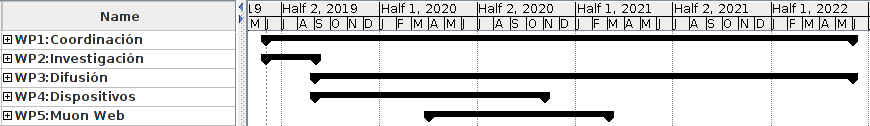
\includegraphics[scale=0.5]{Fotos/GanttWP.png}
						\caption{\label{Img:GanttWP}Diagrama de Gantt de los diferentes paquetes de trabajo WP.}
					\end{figure}

				En la Figura \ref{Img:GanttAll} se muestra el diagrama de Gantt de los diferentes paquetes de trabajo WP detallado de cada tarea. Para ello se ha utilizado el programa \textit{ProjectLibre}.

					\newpage
					\begin{figure}[H]
						\centering
						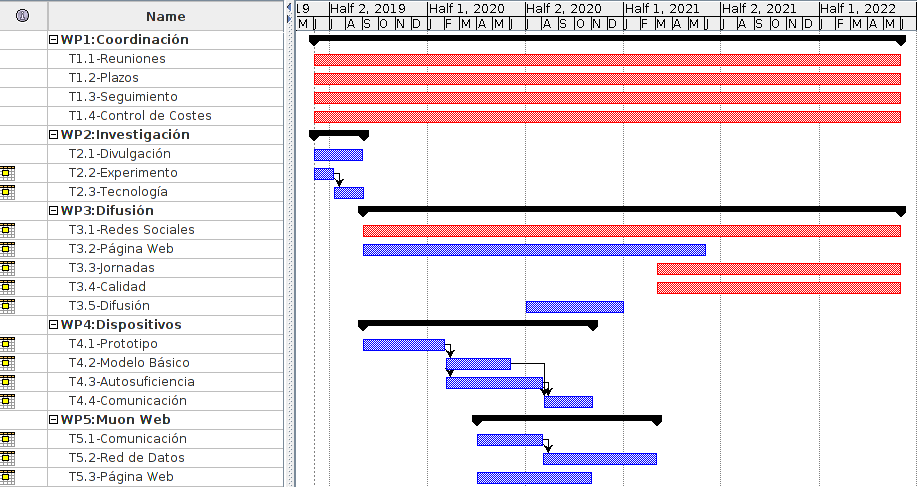
\includegraphics[angle=90, scale=0.65]{Fotos/GanttAll.png}
						\caption{\label{Img:GanttAll}Diagrama de Gantt detallado de los WP con sus tareas.}
					\end{figure}
					\newpage

			\subsection{Información sobre los participantes}
				\addtocontents{toc}{\vspace{0.1cm}}
				\label{SubSec:}

				El grupo que desarrollará el proyecto estará formado por dos estudiantes del último curso de física, que se prevee que durante la realización del proyecto ya hayan concluido su grado en física, y cuatro empleados del Instituto de Física de Cantabria seleccionados según las necesidades del proyecto.

				\begin{itemize}
					\item \textbf{Jaime Díez González-Pardo} Estudiante del cuarto curso del grado en física por la mención de fundamental en la Universidad de Cantabria, 21 años. Se familiarizó con el experimento de la medida de la vida media del muon durante sus prácticas de verano en el \textbf{IFCA}, en las que desarrollo el programa de adquisición de datos del experimento. Coordinador del proyecto. 

					\item \textbf{Marcos Seror García} Licenciado en física y con un máster en divulgación científica, 31 años. Actualmente trabaja en el departamento de divulgación del \textbf{IFCA}.

					\item \textbf{Patricia Martínez Ruiz del Haya} Doctora en física por la Universidad de Cantabria. Actualmente trabaja en el experimento CMS del CERN y es investigadora Ramón y Cajal en el \textbf{IFCA}. Además, es la encargada de impartir la práctica de la medida de la vida media del muon en la Universidad de Cantabria 
					
					\item \textbf{Laura Lloret Iglesias} Doctora en física por la Universidad de Oviedo y el CERN. Actualmente trabaja en el \textbf{IFCA} y es responsable academica del master de Data Science de la UIMP-UC.

					\item \textbf{Roberto Vilar Cortale} Doctor en física y miembro del grupo de altas energías del \textbf{IFCA}, vicedirector del \textbf{IFCA} y resposable de divulgación del mismo. Además, años atrás ha sido el responsable de dicho experimento en la Universidad de Cantabria hasta la llegada de Patricia Martínez Ruiz del Haya.

					\item \textbf{Daniela Iglesias Sánches} Estudiante del cuarto curso del grado en física por la mención de aplicada en la Universidad de Cantabria, 21 años. Tiene conocimientos altos en lenguajes de programación orientados al desarrollo web como javascript.
				\end{itemize}

				Los participantes del proyecto han sido seleccionados teniendo en cuenta las características necesarias para su desarrollo. De esta forma se ha logrado un grupo de participantes reducido pero en el que cada miembro aporta una cualidad diferente al proyecto.

				Por un lado, cabe destacar la participación de tres Doctores/as en física con gran actividad en el CERN, así como la de los dos responsables actualmente de la divulgación del \textbf{IFCA}.También es importante destacar la presencia de tres miembros que ya han trabajado en el experimento y cuyo conocimiento del mismo es muy valioso de cara a la realización del proyecto. Por otro lado, el grupo cuenta con un gran conocimiento de los seervicios informaticos básicos necesarios para llevar a cabo las diferentes tareas del proyecto.

				Por último, junto con la experincia y conocimiento de los investigadores del \textbf{IFCA} se encuentra la juventud de los dos estudiantes de física, que pueden dar otro enfoque, junto con Marcos Seror García, de cara a la divulgación del experimento a jovenes.

				\subsubsection{Tareas y responsabilidades de los participantes}
					\addtocontents{toc}{\vspace{0.1cm}}
					\label{SubSec:}

					\begin{table}[H]
					    \centering
						\begin{tabular}{m{4.5cm} m{2.5cm} m{0.4cm} m{0.4cm} m{0.4cm} m{0.4cm} m{0.4cm} m{0.4cm}}
							\hline
							\multicolumn{1}{m{4.5cm}}{\centering \textbf{Tareas}} &  
							\multicolumn{1}{m{2.5cm}}{\centering \textbf{Responsable}} &
							\multicolumn{1}{m{1.cm}}{\centering \textbf{JDGP}} &
							\multicolumn{1}{m{1.cm}}{\centering \textbf{MSG}} &
							\multicolumn{1}{m{1.cm}}{\centering \textbf{PMRH}} &
							\multicolumn{1}{m{1.cm}}{\centering \textbf{LLI}} &
							\multicolumn{1}{m{1.cm}}{\centering \textbf{RVC}} &
							\multicolumn{1}{m{1.cm}}{\centering \textbf{DIS}} \\ \hline
						   	\hline
						   	WP1: Coordinación 		& JDGP 	&	& 	& 	& 	&	&   \\ \hline
						    T 1.1 Reuniones 		& 		&	& 	& P	& P	& P	&   \\ \hline
						    T 1.2 Plazos 			& 		&	& 	& P	& P	& P	&   \\ \hline
						    T 1.3 Seguimiento 		& 		&	& 	& P	& P	& P	&   \\ \hline
						    T 1.4 Control de costes & 		&	& 	& P	& P	& P	&   \\ \hline
						    WP2: Investigación 		& PMRH 	&	& 	& 	& 	&	&   \\ \hline
						    T 2.1 Divulgación 		& 		& P	& P	& 	& 	& P	&   \\ \hline
						    T 2.2 Experimento 		& 		& P	& 	& 	& 	&	&   \\ \hline
						    T 2.3 Tecnología 		& 		& P	& 	& 	& P	&	& P \\ \hline
						    WP3: Difusión 			& RVC 	&	& 	& 	& 	&	&   \\ \hline
						    T 3.1 Redes Sociales 	& 		&	& P	& 	& 	& P	&   \\ \hline
						    T 3.2 Página Web 		& 		&	& P	& 	& 	&	& P \\ \hline
						    T 3.3 Jornadas 			& 		& I	& P	& I	& 	& P	&   \\ \hline
						    T 3.4 Difusión 			& 		&	& P	& 	& 	& P	&   \\ \hline
						    WP4: Dispositivo 		& JDGP 	&	& 	& 	& 	&	&   \\ \hline
						    T 4.1 Prototipo 		& 		&	& 	& P	& 	&	&   \\ \hline
						    T 4.2 Modelo Básico 	& 		&	& 	& P	& 	&	&   \\ \hline
						    T 4.3 Autosuficiencia 	& 		&	& 	& P	& 	&	&   \\ \hline
						    T 4.4 Comunicación 		& 		&	& 	& P	& I	&	& I \\ \hline
						    WP5: Muon Web 			& LLI 	&	& 	& 	& 	&	&   \\ \hline
						    T 5.1 Comunicación 		& 		&	& 	& I	& 	&	& P \\ \hline
						    T 5.2 Red de Datos 		& 		&	& 	& 	& 	&	& P \\ \hline
						    T 5.3 Página Web 		& 		&	& 	& 	& 	&	& P \\ \hline
					    \end{tabular}
					    \caption{\label{tab:Tareas} Tabla con la participación de cada miembro en las tareas del proyecto. P=participación directa, I=Informado}
					\end{table}

		\section{Gestión Económica}
			\addtocontents{toc}{\vspace{0.1cm}}
			\label{Sec:}

			\subsection{Presupuesto}
				\addtocontents{toc}{\vspace{0.1cm}}
				\label{SubSec:}

				Puesto que el proyecto se pretende englobar dentro de las actividades de divulgación del Instituto de Física de Cantábria, se espera contar para el presupuesto del proyecto con la financiación por parte de éste. Además, se solicitarán diversas becas para la divulgación científica existentes, como la convocatoria de ayudas para el fomento de la cultura científica, tecnológica y de la innovación \cite{FECYT}, siendo esta parte el bloque centras de la financiación.

				Por otra parte, el \textbf{IFCA} aportará al proyecto los recursos humanos necesarios para su desasrrollo. Dentro de este bloque se incluye a los participantes mencionados que se encuentran actualmente trabajando para el \textbf{IFCA}.

			\subsection{Recursos materiales necesarios}
				\addtocontents{toc}{\vspace{0.1cm}}
				\label{SubSec:}

				El proyecto requerirá de la fabricación de dos dispositivos experimentales que permitan realizar las mediciones necesarias para la realización del experimento. Se desarrollará un modelo básico compuesto por el instrumental necesario para la realización del experimento en aulas. Por otro lado, se desarrollará otro dispositivo más complejo que contará con paneles solares y sistemas de comunicación half-duplex, para el acceso remoto a los datos.

				En la Tabla \ref{tab:Basico} se muestra los componentes necesarios para la fabricación del modelo básico por unidad.

				\begin{table}[H]
					    \centering
						\begin{tabular}{m{3.5cm} m{1.0cm} m{5.4cm}}
							\hline
							\multicolumn{1}{m{3.5cm}}{\centering \textbf{Material}} &  
							\multicolumn{1}{m{1.0cm}}{\centering \textbf{Coste}} &
							\multicolumn{1}{m{5.4cm}}{\centering \textbf{Fabricante}} \\ \hline
						   	\hline
						   	Plástico centelleante	& -	&  Eljen Technology / \url{https://eljentechnology.com/} \\ \hline
						    Fotomultiplicador 		& - &	Hamamatsu / \url{https://www.hamamatsu.com}  \\ \hline
						    Raspberry Pi Zero		& 20 & Amazon \\ \hline
						    Circuito de lectura		& - & - \\ \hline
					    \end{tabular}
					    \caption{\label{tab:Basico} Tabla con la participación de cada miembro en las tareas del proyecto. P=participación directa, I=Informado}
					\end{table}

				En la Tabla \ref{tab:Autonomo} se muestra los componentes necesarios para la fabricación del modelo autónomo por unidad.

				\begin{table}[H]
					    \centering
						\begin{tabular}{m{3.5cm} m{1.0cm} m{5.4cm}}
							\hline
							\multicolumn{1}{m{3.5cm}}{\centering \textbf{Material}} &  
							\multicolumn{1}{m{1.0cm}}{\centering \textbf{Coste}} &
							\multicolumn{1}{m{5.4cm}}{\centering \textbf{Fabricante}} \\ \hline
						   	\hline
						   	Plástico centelleante (EJ-212)	& -	&  Eljen Technology / \url{https://eljentechnology.com/} \\ \hline
						    Fotomultiplicador 		& - &	Hamamatsu / \url{https://www.hamamatsu.com}  \\ \hline
						    Raspberry Pi Zero		& 20 & Amazon \\ \hline
						    Circuito de lectura		& - & - \\ \hline
						    Paneles solares			& 100 & Autosolar \url{https://autosolar.es/paneles-solares} \\ \hline
						    Comunicación UHF 		& - & - \\ \hline
					    \end{tabular}
					    \caption{\label{tab:Autonomo} Tabla con la participación de cada miembro en las tareas del proyecto. P=participación directa, I=Informado}
					\end{table}

		\section{Riesgos}
			\addtocontents{toc}{\vspace{0.1cm}}
			\label{Sec:}

			\subsection{Análisis de riesgos y contingencias}
				\addtocontents{toc}{\vspace{0.1cm}}
				\label{SubSec:}

				\begin{table}[H]
					    \centering
						\begin{tabular}{m{5.0cm} m{2.0cm} m{2.0cm} m{5.0cm}}
							\hline
							\multicolumn{1}{m{5.0cm}}{\centering \textbf{Descripción del Riesgo}} &  
							\multicolumn{1}{m{2.5cm}}{\centering \textbf{Probabilidad}} &
							\multicolumn{1}{m{2.4cm}}{\centering \textbf{WP afectados}} &
							\multicolumn{1}{m{4.cm}}{\centering \textbf{Propuesta para mitigarlo}}  \\ \hline
						   	\hline
						   	Fallo en el sistema de autoavastecimiento energético del dispositivo experimental & Media & WP3, WP4 & Se buscaría más apoyo de centros que acogiesen los dispositivos \\ \hline
						    Alto coste de producción de los dispositivos & Bajo & WP1, WP4 & Se buscaría abaratar el dispositivo disminuyendo sus prestaciones, además de la busqueda de nuevas fuentes de financiación \\ \hline
						    Falta de interés por parte de Intitutos & Bajo & WP3 & Se buscaría una nueva via para llegar a los jovenes interesados en las jornadas \\ \hline
						    Falta de interés por parte de los alumnos & Bajo & WP3 & Cambiaar el contenido de las jornadas para hacerlas más atractivas para el alumnado \\ \hline	    
					    \end{tabular}
					    \caption{\label{tab:Tareas} Tabla con la participación de cada miembro en las tareas del proyecto. P=participación directa, I=Informado}
					\end{table}

			\subsection{Análisis DAFO}
				\addtocontents{toc}{\vspace{0.1cm}}
				\label{SubSec:}

					Es importante de cara a la realización del proyecto tener en cuenta los puntos fuertes, debilidades, oportunidades y amenazas que pueda tener el proyecto durante su desarrollo. En la Tabla \ref{tab:Dafo} se muestra el análisis DAFO del proyecto.

					\begin{table}[H]
					    \centering
						\begin{tabular}{||m{7.0cm} | m{7.0cm}||}
							\hline \hline
							\multirow{1}{7.0cm}{\centering \Large \textbf{Fortalezas}} & \multirow{1}{7.0cm}{\centering \Large  \textbf{Debilidades}} \\
							& \\
							Grupo con gran experiencia en la física de partículas  & Proyecto completamente nuevo sustentado en el apoyo de centros externos\\
							Experiencia anterior en actividades de divulgación científica  & Grupo pequeño \\
							Experimento que permite la enseñanza de conceptos de física fundamental a partir de conocimientos básicos & Falta de presupuesto \\
							Participación del centro de investgación \textbf{IFCA} & Dependiencia del autoabastecimiento energético del dispositivo autónomo \\\hline
							\multirow{1}{7.0cm}{\centering \Large \textbf{Oportunidaddes}} & \multirow{1}{7.0cm}{\centering \Large \textbf{Amenazas}} \\
							& \\
							Gran aumento de las actividades de divulgación científica & Falta de apoyo de centros externos \\
							Participación del \textbf{IFCA} en actividades de divulgación y colaboración con el \textbf{IPPOG} & Fallo en los dispositivos remotos \\
							\hline \hline
							%\multicolumn{1}{m{7.0cm}}{\centering \textbf{Descripción del Riesgo}} 
					    \end{tabular}
					    \caption{\label{tab:Dafo} Analisis DAFO del proyecto}
					\end{table}

			\subsection{Matriz de estrategia}
				\addtocontents{toc}{\vspace{0.1cm}}
				\label{SubSec:}

				El análisis de los puntos fuertes y las debilidades del proyecto permite definir las estrategias que se llevarán a cabo. En la Tabla \ref{tab:Estrategias} se muestra la matriz de estrategia desarrollada a partir del análisis DAFO de la Tabla \ref{tab:Dafo}.

					\begin{table}[H]
					    \centering
						\begin{tabular}{||m{3.5cm} | m{5.0cm} | m{5.0cm}||}
							\hline \hline
							\multirow{1}{3.5cm}{\centering \Large \textbf{Estrategias}}  & \multirow{1}{5.0cm}{\centering \Large  \textbf{Fortalezas}} & \multirow{1}{5.0cm}{\centering \Large  \textbf{Debilidades}} \\ 
							& & \\\hline
							\multirow{1}{3.5cm}{\centering \Large \textbf{Oportunidades}} & Ofrecer un nuevo experimento para la divulgación que permita acercar la física de partículas a la divulgación  & Utilizar las recursos y colaboraciones del \textbf{IFCA} con otros centros \\ \hline
							\multirow{1}{3.5cm}{\centering \Large \textbf{Amenazas}} & Ofrecer las actividades del proyecto a los centros en diferentes niveles de implicación y presupuesto & Falta de convencimiento de los centros sobre el éxito y la utilidad de las jornadas de divulgación \\
							\hline \hline
							%\multicolumn{1}{m{7.0cm}}{\centering \textbf{Descripción del Riesgo}} 
					    \end{tabular}
					    \caption{\label{tab:Estrategias} Matriz de estrategia del proyecto realizado a partir del análisis DAFO.}
					\end{table}

%----------------------------------------------------------------------------
%     BIBLIOGRAPHY
%----------------------------------------------------------------------------
	\newpage

	\bibliographystyle{ieeetr}
	\bibliography{biblio}


\end{document}


%----------------------------------------------------------------------------
%            TEMPLATES
%----------------------------------------------------------------------------

%----------------------------------------------------------------------------
%            how to insert an image
%----------------------------------------------------------------------------

%	\begin{figure}[H]
%		\centering
%		\includegraphics[scale= ]{nombre de la imagen.jpg}
%		\caption{\label{Img:widgets}el pie de pagina que le quieras 	poner a la imagen}
%	\end{figure}
 
%----------------------------------------------------------------------------
%            how to insert a table
%----------------------------------------------------------------------------

%	\begin{table}[H]
%		\centering
%		\begin{tabular}{|c|c|c|c|}
%			\hline
%			\centering
%				Altura(h) & Distancia (d) & Elaboracion (e) & Longitud (l) \\
%				($\pm0.5$ mm) & ($\pm0.5$ mm) & ($\pm0.5$ mm) & ($\pm0.5$ mm) \\ \hline
%				 &  &  &  \\ \hline
%				 &  &  &  \\ \hline
%				 &  &  &  \\ \hline
%				 &  &  &  \\ \hline
%				 &  &  &  \\ \hline
%		         &  &  &  \\ \hline
%		\end{tabular}
%		\caption{\label{Tab:widgets}pie de pagina que le quieras poner}
%	\end{table}

%----------------------------------------------------------------------------
%             How to remove the label in equactions
%----------------------------------------------------------------------------

%	\begin{equation*}
%		
%	\end{equation*}

%----------------------------------------------------------------------------
%              How to set bibliography
%----------------------------------------------------------------------------

%\bibliographystyle{unsrt}
%\bibliography{biblio}
%
%Then you have to set a .bib document such as the next template
%
%	@book{nickname,
%	author = {},
%	title = {},
%	edition = {},
%	year = {},
%	volume = {},
%	ISBN = {}
%	}
%
%	@ARTICLE{nickname,
%	author = {},
%	title = {},
%	year = {},
%	volume = {},
%	}


%----------------------------------------------------------------------------
%              END
%----------------------------------------------------------------------------
